\documentclass[11pt,a4paper,oneside]{book}

% ---------------------------------------------------------------------------
% Packages
% ---------------------------------------------------------------------------
\usepackage[margin=2.5cm]{geometry}
\usepackage[utf8]{inputenc}
\usepackage[T1]{fontenc}
\usepackage{graphicx}
\usepackage{tikz}
\usetikzlibrary{shapes.geometric, arrows.meta, positioning, fit, backgrounds, calc}
\usepackage{booktabs}
\usepackage{xcolor}
\usepackage{hyperref}
\usepackage{listings}
\usepackage{enumitem}
\usepackage{caption}
\usepackage{float}
\usepackage{parskip}
\usepackage{underscore}
\usepackage[export]{adjustbox}
\usepackage{amsmath}
\usepackage{longtable}

\hypersetup{
    colorlinks=true,
    linkcolor=blue!50!black,
    citecolor=blue!50!black,
    urlcolor=blue!50!black,
    pdftitle={A Query Recommender for Preference-Aware Natural Language Querying over Virtual Knowledge Graphs},
    pdfauthor={Narges}
}

% ---------------------------------------------------------------------------
% One consistent color palette, reused by every diagram in this thesis
% (deliberately unified across chapters, unlike the standalone per-phase
% reports this document draws on, each of which had its own local palette).
% ---------------------------------------------------------------------------
\definecolor{colSource}{RGB}{215,235,250}   % data sources / stores (blue)
\definecolor{colGreen}{RGB}{225,245,225}    % "actual" / retrieval / already-built
\definecolor{colOrange}{RGB}{255,235,205}   % "stated" / generation / external interfaces
\definecolor{colPurple}{RGB}{240,225,245}   % pipeline / processing stages
\definecolor{colPink}{RGB}{255,225,225}     % outputs / ranking / harness
\definecolor{colBorder}{RGB}{80,80,80}

\tikzset{
    block/.style={rectangle, draw=colBorder, rounded corners, thick,
        text width=3.2cm, minimum height=1.1cm, align=center, font=\small},
    smallblock/.style={rectangle, draw=colBorder, rounded corners, thick,
        text width=2.6cm, minimum height=0.9cm, align=center, font=\footnotesize},
    arrow/.style={-{Latex[length=2.5mm]}, thick}
}

% ---------------------------------------------------------------------------
% Listings style
% ---------------------------------------------------------------------------
\lstset{
    basicstyle=\ttfamily\footnotesize,
    breaklines=true,
    frame=single,
    backgroundcolor=\color{gray!7},
    columns=fullflexible,
    showstringspaces=false,
    xleftmargin=1em,
    xrightmargin=1em,
    aboveskip=8pt,
    belowskip=8pt
}

\newcommand{\code}[1]{\texttt{#1}}

\begin{document}

% =============================================================================
\begin{titlepage}
\centering
\vspace*{2cm}

{\Large \scshape (University name / department --- to be filled in from the official
department template) \par}

\vspace{2.5cm}

{\Huge \bfseries A Query Recommender for Preference-Aware\\[4pt] Natural Language Querying over\\[4pt] Virtual Knowledge Graphs \par}

\vspace{1.5cm}

{\Large A behavior-aware, retrieval-augmented recommender that conditions follow-up query\\
suggestions on both a user's stated queries and their real interaction behavior \par}

\vspace{3cm}

{\large
\begin{tabular}{ll}
\textit{Author:} & Narges \\[6pt]
\textit{Supervisor:} & Prof. Elisa Quintarelli \\
\end{tabular}
\par}

\vfill

{\large Master's Thesis \par}
{\large \today \par}

\end{titlepage}

% =============================================================================
\frontmatter

\chapter*{Abstract}
\addcontentsline{toc}{chapter}{Abstract}

The baseline system this thesis extends, ``Indeewari,'' lets a non-expert user type a
natural-language question (e.g.\ \emph{``Churches in Verona''}) and receive results retrieved from
a Virtual Knowledge Graph (VKG) via an LLM-driven NL2SPARQL pipeline. This thesis addresses a gap
its own predecessor paper names explicitly as future work: the system answers a question but never
helps the user ask a \emph{better} next one. The contribution is a \textbf{query recommender} ---
delivered as a standalone model and API, not a UI feature --- that, after a query is answered,
proposes three follow-up query suggestions.

The central research idea, attributed by the supervisor to ``Jerry's'' analysis, is that a user's
\emph{stated} queries and their \emph{real} interaction behavior often diverge: a user may type
\emph{``romantic movie''} but consistently watch American comedies. A recommender conditioning on
query history alone is, on this view, little more than autocomplete. This thesis builds and
evaluates a recommender that conditions on \emph{both} signals. A per-user behavioral preference
profile is constructed from real (synthetic but behaviorally rich) watch and search data,
quantifying how far a user's stated search intent diverges from what they actually watch. This
signal is injected into a retrieval-augmented generation pipeline, adapted from the GQR/RA-GQR
line of work: an LLM proposes candidate follow-up queries conditioned on the user's retrieved past
queries \emph{and} their behavioral divergence, candidates are passed through a schema-grounding
validation step to mitigate hallucinated, unanswerable suggestions, and a final ranking stage
scores and diversifies the result along two axes echoing the classical query-recommendation
literature: lexical similarity to query history versus alignment with real behavior.

A controlled ablation --- the real production pipeline run twice per (user, question) pair, once
with and once without the behavioral signal, scored identically against real held-out ground truth
--- shows that conditioning on behavior increases behavioral-alignment@3 by roughly $6.5\times$ and
proxy-recall@3 by more than $2\times$, consistently across every evaluated user and question. This
is the thesis's central empirical result: conditioning candidate generation and ranking on real
interaction behavior, not just stated query text, measurably shifts suggestions toward what a user
actually engages with. The system, its design rationale, an empirically-grounded limitation in
schema-grounding validation, and this evaluation are the subject of the chapters that follow.

\tableofcontents
\listoffigures
\listoftables

\chapter*{Abbreviations}
\addcontentsline{toc}{chapter}{Abbreviations}

\begin{tabular}{ll}
VKG      & Virtual Knowledge Graph \\
OBDA     & Ontology-Based Data Access \\
NL2SPARQL & Natural-Language-to-SPARQL translation \\
LLM      & Large Language Model \\
GQR      & Generating Query Recommendations (via LLMs) \\
RA-GQR   & Retrieval-Augmented GQR \\
SHACL    & Shapes Constraint Language \\
MMR      & Maximal Marginal Relevance \\
API      & Application Programming Interface \\
JSON     & JavaScript Object Notation \\
SQL      & Structured Query Language \\
\end{tabular}

% =============================================================================
\mainmatter

% =============================================================================
\chapter{Introduction}
\label{ch:intro}
% =============================================================================

\section{Motivation and Problem Statement}
\label{sec:intro-motivation}

Virtual Knowledge Graphs (VKGs) let a relational database be queried as if it were RDF, through an
Ontology-Based Data Access (OBDA) mapping layer such as Ontop~\cite{ontop}. Combined with an
LLM-driven natural-language-to-SPARQL (NL2SPARQL) pipeline, this lets a non-expert user ask a
question in plain language --- \emph{``Churches in Verona''} --- and receive results retrieved
directly from the underlying data, with no SPARQL expertise required. This is the architecture of
the baseline system this thesis extends, ``Indeewari''~\cite{balasooriya2026}, developed under the
same supervisor and grounded in the Verona tourism domain.

The supervisor's own paper describing that baseline system explicitly names
\emph{``recommendations''} as future work~\cite{balasooriya2026}: the system answers a question but
does nothing to help a user formulate a better next one. An email from the supervisor made this
concrete, asking for three extensions, in increasing order of research weight:

\begin{enumerate}[label=(\arabic*)]
    \item \textbf{Domain selection} --- generalize the application so a user can choose \emph{which}
        VKG to query (e.g.\ Movie vs.\ Tourism) instead of the system being wired to a single
        dataset.
    \item \textbf{User selection instead of login} --- let the user pick \emph{who they are} from a
        list of personas, so the system can reason about that user's preferences, without
        implementing real authentication.
    \item \textbf{Query recommendation} --- the thesis's core contribution: after answering a
        query, propose three follow-up query suggestions. If a user asks \emph{``Churches in
        Verona,''} the system should show results \emph{plus} suggestions such as \emph{``Roman
        Churches in Verona,''} \emph{``Free Churches in Verona,''} or \emph{``Trip to visit churches
        in Verona.''} Critically, this recommender should consider not only the user's previous
        queries but also their \textbf{real interaction data} --- because what a user \emph{says}
        they want and what they \emph{actually} engage with are frequently different.
\end{enumerate}

Item (3) is this thesis's actual contribution, and its framing is the thesis's central research
question: can a recommender that conditions on both a user's stated queries \emph{and} their real
interaction behavior produce suggestions that are measurably better --- more aligned with what the
user actually wants --- than one conditioning on query history alone?

\section{Scope of This Thesis}
\label{sec:intro-scope}

Following an email exchange with the supervisor, after items (1) and (2) had already been partially
explored, the scope was narrowed. Domain selection and user selection instead of login are handled
by a separate application, already implemented by two other students under the same supervisor,
described by the supervisor as ``empty on the recommendation side.'' This thesis does not build or
integrate with that application's user interface. Its entire contribution is item (3): the query
recommender, delivered as a \textbf{standalone model and API} --- any calling application,
including the other students' system, integrates it later by calling an endpoint. This thesis is
not responsible for that integration.

The multi-domain VKG infrastructure that had already been built at the time of this scope decision
--- two working VKGs (Movie and Tourism) and a domain-switching development harness --- is retained,
but strictly as an \textbf{internal development and evaluation harness}: a way to build, test, and
demo the recommender against real schemas and data, without depending on the external
application's timeline or codebase. It is documented in Chapter~\ref{ch:arch} because the
recommender's schema-grounding step and one of its two evaluation domains depend on it, but it is
explicitly not, itself, a thesis deliverable.

\section{Contributions}
\label{sec:intro-contrib}

This thesis makes the following contributions:

\begin{itemize}
    \item A \textbf{per-user behavioral preference profile} (Chapter~\ref{ch:behavior}) that
        quantifies, for the Movie domain, how far a user's stated search intent diverges from what
        they actually watch --- including an engineered temporal-join heuristic recovering an
        implicit link between free-text search queries and later watch events that does not exist
        as a key in the source data.
    \item A \textbf{retrieval-augmented, behavior-conditioned query recommender}
        (Chapter~\ref{ch:recommender}) --- a four-stage pipeline (retrieval, LLM-based candidate
        generation, schema-grounding validation, and behavior-aware ranking) delivered as a
        standalone HTTP API, adapting the GQR/RA-GQR line of work~\cite{bacciu2024} and borrowing
        scoring-axis ideas from classical, non-LLM query-recommendation research~\cite{barman2024}.
    \item An \textbf{empirically-grounded negative result} on schema-grounding validation
        (Section~\ref{sec:rec-validation}): a precision hallucination filter, motivated directly by
        a documented risk in the LLM+KG integration literature~\cite{pan2024} and by the baseline
        system's own measured SPARQL-correctness rate~\cite{balasooriya2026}, was designed,
        calibrated, and found not to be achievable with acceptable precision given how sparse this
        project's source ontologies are --- a concrete, reportable limitation rather than a silently
        shipped, over-claimed feature.
    \item A \textbf{controlled ablation study} (Chapter~\ref{ch:eval}) isolating the effect of the
        behavioral signal on suggestion quality, scored against real held-out ground truth, showing
        a $6.5\times$ increase in behavioral-alignment@3 and a more than $2\times$ increase in
        proxy-recall@3 when the behavioral profile is included --- the thesis's central empirical
        confirmation that conditioning on real behavior, not just stated query text, produces
        measurably different and better-aligned recommendations.
\end{itemize}

\section{Thesis Structure}
\label{sec:intro-outline}

Chapter~\ref{ch:relwork} reviews the four bodies of literature that ground the recommender's
design. Chapter~\ref{ch:arch} describes the system architecture and development harness the
recommender is built and evaluated against. Chapter~\ref{ch:behavior} presents the behavioral
preference profile, the empirical substrate for the thesis's central premise.
Chapter~\ref{ch:recommender} presents the recommender core itself --- the thesis's central design
contribution. Chapter~\ref{ch:eval} presents the evaluation and its results.
Chapter~\ref{ch:conclusion} summarizes the contributions, discusses limitations, and outlines
future work.

% =============================================================================
\chapter{Related Work}
\label{ch:relwork}
% =============================================================================

Four bodies of work ground the design decisions made in this thesis, each informing a different
part of the system.

\section{Natural Language Reasoning over Virtual Knowledge Graphs}
\label{sec:rel-nl2sparql}

Balasooriya, Dalla Vecchia, and Quintarelli~\cite{balasooriya2026} describe the baseline system
this thesis extends: Ontop exposes relational Verona tourism data as a VKG; NL2SPARQL translation
is delegated to SPARQL-LLM, an external, triplestore-agnostic, metadata-driven Text2SPARQL system
using SHACL-annotated query examples, VoID schema descriptions, and embedding-based retrieval; and
a GPT-4.1-mini prompt-based intent classifier first decides whether a question is factual (routed
to NL2SPARQL) or analytical/preference-oriented (routed to a lightweight, frequency-based inference
module over Verona Card visit data). Their preliminary evaluation reports 100\% routing accuracy on
50 hand-labeled questions, but only 70\% SPARQL-correctness on the factual subset --- 12 of 40
failures attributed to entity-linking errors or invalid syntax. Their conclusion explicitly names
recommendations as future work; this thesis is that future work, generalized to a second domain and
grounded in real interaction data rather than only aggregate frequency.

Three design implications follow directly. First, the existing pipeline's stage-by-stage structure
is kept intact; this thesis adds a new module operating \emph{after} result formatting, rather than
replacing the NL2SPARQL core (Chapter~\ref{ch:arch}). Second, their intent-routing pattern --- an
LLM classifying before acting --- is a template this thesis does not directly reuse, but their
70\% SPARQL-correctness figure is a direct, empirically-grounded warning: entity-linking and query
validity are real failure modes, and any downstream step that generates \emph{new} natural-language
queries inherits an analogous risk that they might not be answerable at all
(Section~\ref{sec:rec-validation}).

\section{LLM-Based Query Recommendation}
\label{sec:rel-gqr}

Bacciu, Palumbo, Damianou, Tonellotto, and Silvestri~\cite{bacciu2024} reframe query recommendation
as a pure generation task: prompt an LLM with a handful of \emph{query $\to$ recommendations}
example pairs plus the user's current query, and let the model generate recommendations directly,
with no query-log-trained ranking model needed --- solving the cold-start problem that afflicts
classical, log-mining recommenders. Their RA-GQR variant retrieves semantically similar past
queries from a log via sentence embeddings and approximate nearest-neighbor search, and uses those,
rather than generic hand-curated examples, to build the few-shot prompt dynamically --- Retrieval-
Augmented Generation applied to the recommendation prompt itself. In their experiments, RA-GQR
measurably outperforms plain GQR (roughly $+13$ to $+22\%$ NDCG@10).

This is the direct technique behind Section~\ref{sec:rec-retrieval} and~\ref{sec:rec-generation}: a
prompt is built from (i) a small number of retrieved, embedding-similar past queries from the
user's own log, (ii) the current query, and (iii) an instruction to continue with recommendations,
following their prompt template structure. Their evaluation protocols and metrics --- scoring a
recommendation as if it substituted for the original query, or as if it were appended to it, plus
a blind user-preference study --- are the direct ancestor of this thesis's own ablation design in
Chapter~\ref{ch:eval}, adapted to a query-history-versus-behavioral-profile axis in place of their
original data-availability axis.

\section{LLM and Knowledge Graph Integration}
\label{sec:rel-kgllm}

Pan, Luo, Wang, Chen, Wang, and Wu~\cite{pan2024} survey a broad taxonomy of LLM+KG integration
patterns. Two parts are directly relevant here, not the full taxonomy: their KG-prompting/KGQA
sections describe patterns for injecting retrieved graph facts into an LLM prompt so it reasons
\emph{with} the graph rather than purely from parametric knowledge, informing how this thesis's
recommended queries should ideally be grounded in the loaded ontology's actual classes and
properties rather than an imagined schema; and their repeated, explicit documentation of a
hallucination/faithfulness risk --- that LLM-generated content referencing structured knowledge
must match the target graph \emph{exactly}, and that this remains a known failure mode even with
in-context learning. Combined with the baseline system's own measured 70\% SPARQL-correctness rate
(Section~\ref{sec:rel-nl2sparql}), this directly motivates \emph{not} shipping raw LLM-suggested
queries to a user without first checking that they are actually answerable against the currently
loaded schema --- the requirement Section~\ref{sec:rec-validation} attempts, and partially fails,
to satisfy.

\section{Classical, Non-LLM Query Recommendation}
\label{sec:rel-qrmoccga}

Barman, Sarkar, and Chowdhury~\cite{barman2024} model query recommendation as multi-objective
optimization over a query-click bipartite graph built from search logs, using two objective
functions built from four concrete similarity features --- compound click probability, Jaccard
index of clicked links, Jaccard index of query words, and longest-common-subsequence ratio of query
strings --- optimized via a cooperative co-evolutionary genetic algorithm (QRMOCCGA), evaluated
against SimRank, Heat Diffusion, and commercial search engines on real AOL query logs.

Reimplementing their full cooperative co-evolutionary genetic algorithm is out of scope for this
thesis, but two of its ideas are directly useful and were borrowed at negligible cost. First, their
behavioral-similarity features --- word-overlap and click-overlap similarity between two queries ---
are a simple, non-LLM way to quantify ``how well does this candidate query match the user's actual
watch behavior,'' used directly inside this thesis's own ranking step
(Section~\ref{sec:rec-ranking}) without training anything. Second, their explicit two-objective
framing --- semantic relevance versus lexical/visual similarity --- is the direct conceptual
ancestor of this thesis's own two ranking axes, query-history similarity versus behavioral
alignment, even though the actual ranking mechanism here is a simple weighted score with greedy
diversification rather than a genetic algorithm. QRMOCCGA's simpler feature set is also used
directly as a classical, non-LLM baseline in this thesis's evaluation (Section~\ref{sec:eval-results}).

\section{Positioning of This Thesis}
\label{sec:rel-position}

No prior work reviewed here combines all three ingredients this thesis's recommender uses jointly:
retrieval-augmented, LLM-based candidate generation (from GQR/RA-GQR); an explicit, per-user
divergence signal between stated and actual preference, rather than either signal alone (motivated
directly by the supervisor's framing and absent from all four reviewed papers); and a
schema-grounding validation step informed by, but going beyond, generic LLM+KG hallucination
concerns, calibrated empirically against this project's own ontologies rather than assumed to work.
The negative empirical result reported in Section~\ref{sec:rec-validation} --- that class-level
embedding similarity cannot reliably separate on-topic from off-topic candidates when source
ontology metadata is this sparse --- is, to the author's knowledge, not previously documented in
this specific combination of techniques, and is offered as a concrete, reportable finding for
future work in this space to build on.

% =============================================================================
\chapter{System Architecture and Development Harness}
\label{ch:arch}
% =============================================================================

This chapter describes the infrastructure the recommender (Chapters~\ref{ch:behavior}
and~\ref{ch:recommender}) is built and evaluated against: two running Virtual Knowledge Graphs, a
domain-switching development harness, and the recommender's own API contract and persistence
layer. As established in Section~\ref{sec:intro-scope}, none of this chapter's content is itself a
thesis deliverable --- domain and user selection are the responsibility of a separate, external
application. This chapter is included because the recommender genuinely depends on parts of it: the
schema-grounding validation step (Section~\ref{sec:rec-validation}) consumes the machine-readable
schema representations produced here, one of the two evaluation domains (Tourism,
Section~\ref{sec:eval-results}) is only reachable through this infrastructure, and the API contract
described in Section~\ref{sec:arch-api} is the boundary the recommender core is built inside.

\section{Overview}
\label{sec:arch-overview}

Before this work, the NL2SPARQL pipeline queried a single, hardcoded SPARQL endpoint with no
notion of alternate domains, and had no concept of user identity or query persistence. Three layers
were added on top of the unmodified pipeline core: a containerized data/infrastructure layer
(Section~\ref{sec:arch-vkgs}), a domain registry and switching mechanism used only by the internal
development harness (Section~\ref{sec:arch-domain}), and the recommender's own API contract and
query log (Section~\ref{sec:arch-api}), which is the actual thesis-relevant boundary. Because the
NL2SPARQL pipeline's internals --- schema formatting, class/property relevance extraction, entity
linking, SPARQL generation, execution, and result formatting --- are entirely unmodified, any defect
introduced by this work is necessarily located in the new infrastructure, not in query-answering
logic that predates this thesis.

\section{Two Virtual Knowledge Graphs}
\label{sec:arch-vkgs}

Two domains were stood up as isolated Docker Compose stacks, each a relational database container
feeding an Ontop container exposing the data as a VKG over SPARQL (Figure~\ref{fig:arch-phase0}).

\definecolor{dbcolorA}{RGB}{215,235,250}
\definecolor{ontopcolorA}{RGB}{255,235,205}
\definecolor{regcolorA}{RGB}{255,225,225}
\tikzset{blockA/.style={rectangle, draw=colBorder, rounded corners, thick, text width=3.1cm, minimum height=1.1cm, align=center, font=\small}}
\tikzset{smallblockA/.style={rectangle, draw=colBorder, rounded corners, thick, text width=2.5cm, minimum height=0.9cm, align=center, font=\footnotesize}}

\begin{figure}[H]
\centering
\begin{adjustbox}{max width=0.85\textwidth, max totalheight=0.7\textheight, center}
\begin{tikzpicture}[node distance=1.4cm and 2cm]

    \node[blockA, fill=colSource] (pgm) {\code{postgres-movie}\\[2pt]\footnotesize db: \code{netflix\_vkg}\\ port 5433};
    \node[blockA, fill=colOrange, right=of pgm] (om) {\code{ontop-movie}\\[2pt]\footnotesize port 8081};

    \node[blockA, fill=colSource, below=of pgm] (pgt) {\code{postgres-tourism}\\[2pt]\footnotesize db: \code{tourismdb} (PostGIS)\\ port 5434};
    \node[blockA, fill=colOrange, right=of pgt] (ot) {\code{ontop-tourism}\\[2pt]\footnotesize port 8082};

    \node[smallblockA, fill=colPink, below right=1.0cm and -0.3cm of pgt] (jdbc) {\code{docker\slash{}jdbc\slash{}postgresql.jar}\\[2pt]\footnotesize bind-mounted into both Ontop containers};

    \draw[arrow] (pgm) -- node[above,font=\scriptsize]{healthy} (om);
    \draw[arrow] (pgt) -- node[above,font=\scriptsize]{healthy} (ot);
    \draw[arrow, dashed] (jdbc) -- (om);
    \draw[arrow, dashed] (jdbc) -- (ot);

\end{tikzpicture}
\end{adjustbox}
\caption{Docker Compose topology for the two Virtual Knowledge Graphs. Each Ontop container waits
for its database's healthcheck before starting, and both mount the same JDBC driver directory
(dashed arrows) --- a workaround for a missing-driver defect in the base Ontop image.}
\label{fig:arch-phase0}
\end{figure}

\subsection{The Movie domain}

The Movie side uses a synthetic, Faker-generated Netflix-shaped dataset chosen specifically because
it carries per-user behavioral signals (watch history, search logs, reviews) the Tourism domain
lacks --- the substrate Chapter~\ref{ch:behavior} depends on. \code{postgres-movie} is initialized
from six tables (Table~\ref{tab:arch-movie-tables}); no table has a primary key, since the source
dataset contains genuine duplicate id values across every table, a deliberate accommodation rather
than an oversight.

\begin{table}[H]
\centering
\begin{tabular}{lrl}
\toprule
\textbf{Table} & \textbf{Rows} & \textbf{Role} \\
\midrule
\code{movies}              & 1{,}040   & Catalog \\
\code{users}               & 10{,}300  & User master data \\
\code{watch\_history}       & 105{,}000 & Real behavior (implicit feedback) \\
\code{search\_logs}         & 26{,}500  & Stated intent (free-text search) \\
\code{reviews}             & 15{,}450  & Explicit stated opinions \\
\code{recommendation\_logs} & 52{,}000  & System-suggested vs.\ consumed \\
\bottomrule
\end{tabular}
\caption{Movie-domain tables, with row counts verified exactly against the source CSVs.}
\label{tab:arch-movie-tables}
\end{table}

The pre-existing OBDA mapping for this domain required two categories of fixes before it was usable:
a bug fix (a mapping selected a non-existent column, \code{watch\_duration}, where the real column
is \code{watch\_duration\_minutes}), and a coverage extension --- to 17 mappings in total --- adding
the columns a later phase's search-to-watch temporal join needs (\code{search\_date},
\code{watch\_date}, \code{action}, \code{device\_type}), plus a new object property connecting
\code{WatchSession} to \code{User} that had not previously existed despite the equivalent
\code{WatchSession}$\to$\code{Movie} relationship being present.

\subsection{The Tourism domain}

The Tourism side reuses a real, 293\,MB production PostgreSQL dump of Verona's tourism
application, together with an ontology that --- unlike the Movie domain --- already embeds SHACL
node shapes per class, a direct structural match for the NL2SPARQL pipeline's schema loader
(Section~\ref{sec:arch-domain}). \code{postgres-tourism} runs on a PostGIS-enabled image, since the
source database uses geometry/geography columns a plain Postgres image cannot represent.

\begin{table}[H]
\centering
\begin{tabular}{lr}
\toprule
\textbf{Table} & \textbf{Rows} \\
\midrule
\code{art}      & 41 \\
\code{event}    & 1{,}416 \\
\code{calendar} & 10{,}640 \\
\code{location} & 1{,}600 \\
\bottomrule
\end{tabular}
\caption{Tourism-domain tables, row counts verified exactly against the source backup.}
\label{tab:arch-tourism-tables}
\end{table}

Two mappings in the original OBDA file referenced a table, \code{art\_images}, that does not exist
anywhere in the backup (only a differently-shaped legacy table exists). Rather than reconstructing
the missing table, these two mappings were dropped --- a decision made explicitly with the
supervisor's sign-off, since art images are not needed for this thesis's demonstration. The
resulting classes remain declared in the ontology for documentation purposes but are unpopulated.

\paragraph{An explicit scope decision.} The backup also contains a large behavioral table,
\code{log\_vc} (4.4 million rows of VeronaCard tap-in visits), which could in principle serve as a
Tourism-domain behavioral signal analogous to the Movie domain's watch history. However, it
identifies an anonymous card, not a named person, and the database's only user-like table has just
4 administrative rows, not tourists. It was decided that Tourism stays catalog-query-only for this
thesis: \code{log\_vc} is not mapped into the ontology, and all user-selection/behavior-aware work
in later chapters is carried entirely by the Movie domain. This is a load-bearing scope decision,
not an oversight --- it bounds what Chapters~\ref{ch:behavior},~\ref{ch:recommender},
and~\ref{ch:eval} can demonstrate on the Tourism side, and is referenced repeatedly in those
chapters as the reason certain results are Movie-only.

\section{Domain-Switching Infrastructure}
\label{sec:arch-domain}

A declarative KG registry (\code{kg\_config.yaml}) lists the available knowledge graphs by name,
schema-file path, SPARQL endpoint, and an \code{enabled} flag, read by a small loader function that
returns only enabled entries. This registry, and the internal development harness that consumes it
to let a developer manually switch domains while exercising the recommender, are not thesis
deliverables in themselves (Section~\ref{sec:intro-scope}) and are not documented further here.

One infrastructural fix in this layer is worth recording because it directly affects
Section~\ref{sec:rec-validation}'s later results: the NL2SPARQL pipeline's schema loader builds its
machine-readable schema representation (``m-schema'') entirely from SHACL \code{sh:NodeShape}
triples, with no fallback for plain \code{rdfs:domain}/\code{rdfs:range} declarations. The Movie
ontology, unlike the Tourism ontology, originally had no SHACL shapes at all, so feeding it directly
to the parser silently produced an empty schema (Figure~\ref{fig:arch-shacl}). A one-time conversion
script generates the missing shapes mechanically from the ontology's existing \code{rdfs:domain}
declarations, producing \code{movie\_mschema.json} (11 classes) alongside the Tourism domain's
already-SHACL-native \code{tourism\_mschema.json} (7 classes). Both files are the direct input to
Section~\ref{sec:rec-validation}'s schema-grounding check.

\definecolor{ownercolorB}{RGB}{215,235,250}
\begin{figure}[H]
\centering
\begin{adjustbox}{max width=0.85\textwidth, max totalheight=0.6\textheight, center}
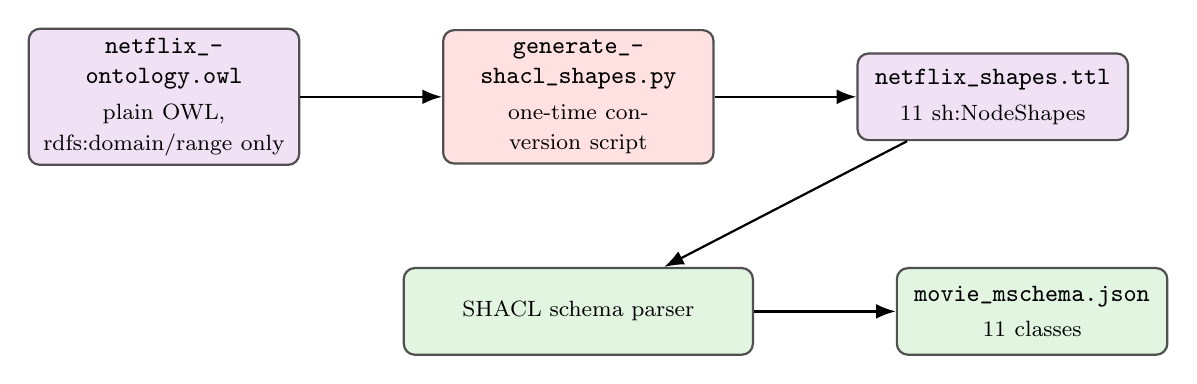
\begin{tikzpicture}[node distance=1.3cm and 1.8cm]
    \node[block, fill=colPurple] (owl) {\code{netflix\_ontology.owl}\\[2pt]\footnotesize plain OWL, rdfs:domain/range only};
    \node[block, fill=colPink, right=of owl] (script) {\code{generate\_shacl\_shapes.py}\\[2pt]\footnotesize one-time conversion script};
    \node[block, fill=colPurple, right=of script] (shapes) {\code{netflix\_shapes.ttl}\\[2pt]\footnotesize 11 sh:NodeShapes};
    \node[block, fill=colGreen, below=of script, text width=4.2cm, font=\footnotesize] (parser) {SHACL schema parser};
    \node[block, fill=colGreen, right=of parser] (mschema) {\code{movie\_mschema.json}\\[2pt]\footnotesize 11 classes};

    \draw[arrow] (owl) -- (script);
    \draw[arrow] (script) -- (shapes);
    \draw[arrow] (shapes) -- (parser);
    \draw[arrow] (parser) -- (mschema);
\end{tikzpicture}
\end{adjustbox}
\caption{The Movie ontology has no native SHACL shapes, so a one-time script generates them from
its existing \code{rdfs:domain}/\code{rdfs:range} declarations before the schema parser can consume
it. This m-schema JSON is the same artifact Section~\ref{sec:rec-validation}'s schema-grounding
check embeds and thresholds against.}
\label{fig:arch-shacl}
\end{figure}

\section{The Recommender API Contract and Query Log}
\label{sec:arch-api}

This is the layer the recommender core (Chapter~\ref{ch:recommender}) is built inside, and the
only genuinely thesis-relevant infrastructure in this chapter beyond the two VKGs above. Before any
recommendation logic exists, two things are needed: a fixed request/response contract external
callers can integrate against, and a place to persist queries, since the recommender's core
technique depends on retrieving a user's own past queries.

\subsection{The contract}

\begin{lstlisting}[language=Python, caption={The recommender's request/response contract. One
field, \code{interaction\_data}, is deliberately left untyped: its real shape depends on what the
external application actually logs per user, a dependency that was never confirmed during this
thesis (Section~\ref{sec:conclusion-limits}).}]
class RecommendRequest(BaseModel):
    user_id: str
    domain: str
    query_text: str
    generated_sparql: Optional[str] = None
    result_summary: Optional[Any] = None
    interaction_data: Optional[dict] = None

class RecommendResponse(BaseModel):
    suggestions: list[str] = Field(default_factory=list)
\end{lstlisting}

\subsection{The query log}

A single SQLite table, indexed on \code{(user\_id, domain)}, appended to on every request. SQLite
was chosen deliberately over a heavier database: a single-file, zero-infrastructure store is
appropriate for a thesis-scale log that does not need to be shared across processes beyond one
local API server, consistent with this project's broader pattern of using the lightest tool that
fits. Two functions cover the read and write side: \code{log\_query()} appends one row (with
automatic JSON-serialization of structured result summaries), and \code{get\_user\_history()}
retrieves the most recent rows for a user, optionally scoped to one domain --- the function
Section~\ref{sec:rec-retrieval}'s retrieval step calls to build its candidate pool.

\subsection{One shared entry point}

Both the real HTTP endpoint (\code{POST /recommend}, exposed via FastAPI, with OpenAPI
documentation auto-served at \code{/docs}) and the internal development harness call a single
function, \code{handle\_recommend()} (Figure~\ref{fig:arch-api}). This was a deliberate design
choice, not a literal reading of the original plan (which could be read as requiring the harness to
make a real HTTP call to a separately-running server): the request/response \emph{shape} being
validated is identical either way, since both paths go through the same pydantic models and the
same handler logic, and requiring a developer to keep a second server process running just to see a
suggestions panel render is friction the contract does not need to impose. External callers are
unaffected by this choice --- they only ever see the HTTP surface.

\definecolor{apicolorC}{RGB}{255,235,205}
\begin{figure}[H]
\centering
\begin{adjustbox}{max width=\textwidth, max totalheight=0.85\textheight, center}
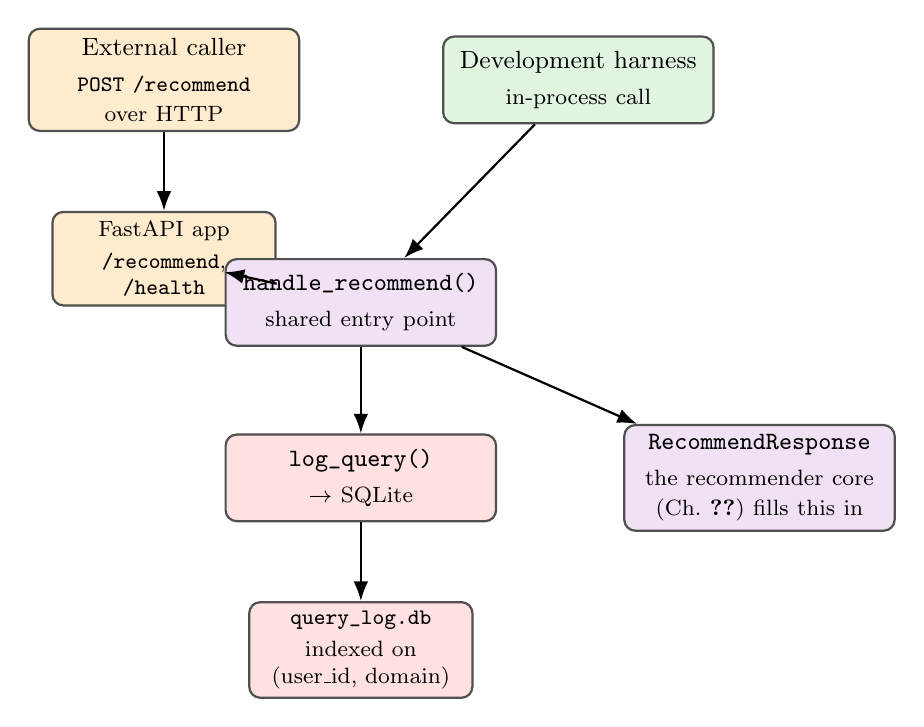
\begin{tikzpicture}[node distance=1.0cm and 1.4cm]

    \node[block, fill=colOrange] (http) {External caller\\[2pt]\footnotesize \code{POST /recommend} over HTTP};
    \node[block, fill=colGreen, right=1.8cm of http] (gui) {Development harness\\[2pt]\footnotesize in-process call};

    \node[smallblock, fill=colOrange, below=of http] (app) {FastAPI app\\[2pt]\footnotesize \code{/recommend}, \code{/health}};

    \node[block, fill=colPurple, below=1.6cm of http, xshift=2.5cm] (handle) {\code{handle\_recommend()}\\[2pt]\footnotesize shared entry point};

    \node[block, fill=colPink, below=1.1cm of handle] (log) {\code{log\_query()}\\[2pt]\footnotesize $\to$ SQLite};

    \node[smallblock, fill=colPink, below=of log] (db) {\code{query\_log.db}\\[2pt]\footnotesize indexed on (user\_id, domain)};

    \node[block, fill=colPurple, right=1.6cm of log] (resp) {\code{RecommendResponse}\\[2pt]\footnotesize the recommender core (Ch.~\ref{ch:recommender}) fills this in};

    \draw[arrow] (http) -- (app);
    \draw[arrow] (app) -- (handle);
    \draw[arrow] (gui) -- (handle);
    \draw[arrow] (handle) -- (log);
    \draw[arrow] (log) -- (db);
    \draw[arrow] (handle) -- (resp);

\end{tikzpicture}
\end{adjustbox}
\caption{Both the real HTTP endpoint and the internal development harness converge on
\code{handle\_recommend()}, which validates the request, persists it, and returns a response. This
is the extension point the recommender core (Chapter~\ref{ch:recommender}) is built inside, without
any further change to the contract, the log store, or the harness.}
\label{fig:arch-api}
\end{figure}

\section{Summary}

This chapter described the infrastructure the recommender depends on but does not itself
contribute: two running VKGs (Movie, behaviorally rich but synthetic; Tourism, real but
catalog-only by explicit scope decision), a domain-switching development harness, and --- the one
piece that is genuinely load-bearing for the thesis --- a fixed API contract and persistent
query log that Chapter~\ref{ch:recommender}'s recommender core is built entirely inside, with no
further change to this boundary.

% =============================================================================
\chapter{Behavioral Preference Profiling}
\label{ch:behavior}
% =============================================================================

\section{Motivation: Stated versus Actual Preference}
\label{sec:behavior-motivation}

The supervisor's framing of the query-recommendation problem rests on a specific empirical claim:
that a user's stated queries and their real interaction behavior often diverge --- a user may type
\emph{``romantic movie''} but consistently watch American comedies. A recommender that only looks
at query history is, per this framing, little more than autocomplete; a genuinely useful one must
condition on both signals. This chapter builds the first half of that requirement: a
machine-readable, per-user summary of what a user says they want versus what they actually engage
with, quantified as a single divergence score. This is the empirical substrate
Chapter~\ref{ch:recommender}'s candidate generation and ranking stages condition on.

This chapter operates on the \textbf{Movie domain only}, for the reason established in
Section~\ref{sec:arch-vkgs}: the Tourism domain's only large behavioral table is keyed to an
anonymous card, not a named user, and was explicitly excluded from the ontology. All
behavior-aware work in this thesis is therefore carried by the Movie domain's dataset (10{,}300
users, 1{,}040 movies, 105{,}000 watch events, 26{,}500 search-log entries).

\section{Method}
\label{sec:behavior-method}

For each user, two independent rankings are computed over the same vocabulary of catalog categories
(genre, content type, country of origin): one derived from what they searched for, one from what
they watched. Three design choices make the resulting comparison meaningful rather than a raw
count comparison.

\subsection{Weighting, not counting}

A watch event a user completed counts more than one abandoned after 5\% of its duration; this is
implemented as a continuous completion weight rather than a binary watched/not-watched signal:

\[
w(\text{row}) =
\begin{cases}
1.0 & \text{if } \code{action} = \code{"completed"} \\[4pt]
\operatorname{clip}\!\left(\dfrac{\code{progress\_percentage}}{100},\, 0.05,\, 1.0\right) &
    \text{if progress is known} \\[8pt]
0.3 & \text{otherwise}
\end{cases}
\]

This operationalizes ``actual interest'' as \emph{how much} of something a user engaged with, not
merely whether a watch event was logged: a user who starts and abandons five thrillers should not
count for as much as one who finishes a single thriller. Weighted watches are grouped by
\code{(user, month, category)} and normalized by that user-month's total weighted interactions to
obtain a relative intensity in $[0,1]$.

\subsection{An engineered link between two unconnected data sources}
\label{sec:behavior-link}

The search-log and watch-history tables share no foreign key in the source dataset --- there is no
column recording which movie, if any, a given search led to. A temporal join recovers this link
where it plausibly exists: for every search with at least one inferred category, the user's next
watch within a 7-day window is found via a forward, tolerance-bounded merge, grouped per user.

\begin{lstlisting}[language=Python, caption={The temporal join. \code{matched\_stated\_intent}
flags whether any category inferred from the search actually appears among the linked watch's own
genre/content-type --- an individually inspectable, row-level artifact of stated-vs-actual
correspondence, independent of the aggregate divergence score in Section~\ref{sec:behavior-divergence}.}]
linked = pd.merge_asof(
    searches, watch_sorted,
    left_on="search_date", right_on="watch_date", by="user_id",
    direction="forward", tolerance=pd.Timedelta(days=7),
    suffixes=("", "_watched"),
)
linked = linked.dropna(subset=["movie_id"]).copy()
linked["matched_stated_intent"] = linked.apply(
    lambda r: bool(set(r["inferred_categories"])
                   & {r["genre_primary"], r["genre_secondary"], r["content_type"]}),
    axis=1,
)
\end{lstlisting}

Which categories a search is tagged with in the first place is not a trivial substring match: an
early implementation let \code{content\_type="Movie"} spuriously match inside the plural word
``movies'' in nearly every query, and would similarly have let \code{"War"} match inside
``warrior.'' The fix, a word-boundary regular expression rather than a plain substring test, is
worth recording as a concrete lesson for any similarly-structured tagging step:

\begin{lstlisting}[language=Python, caption={Word-boundary category tagging, applied to every
search query against a vocabulary sorted longest-string-first so a multi-word value like
``Stand-up Comedy'' is checked before a shorter value like ``Comedy'' could match part of it.}]
def build_vocabulary_patterns(vocabulary):
    return {v: re.compile(r"\b" + re.escape(v.lower()) + r"\b") for v in vocabulary}

def infer_categories(search_query, vocabulary_patterns):
    query = str(search_query).lower()
    return [v for v, pattern in vocabulary_patterns.items() if pattern.search(query)]
\end{lstlisting}

\subsection{A single summary statistic}
\label{sec:behavior-divergence}

Each user's top-5 actual categories and top-5 stated categories, ranked by summed intensity across
all months, are compared via Jaccard similarity: $|A \cap S| / |A \cup S|$ for actual set $A$ and
stated set $S$. This single number is the behavioral divergence signal
Chapter~\ref{ch:recommender}'s candidate generation and ranking condition on.

\begin{figure}[H]
\centering
\begin{adjustbox}{max width=\textwidth, max totalheight=0.85\textheight, center}
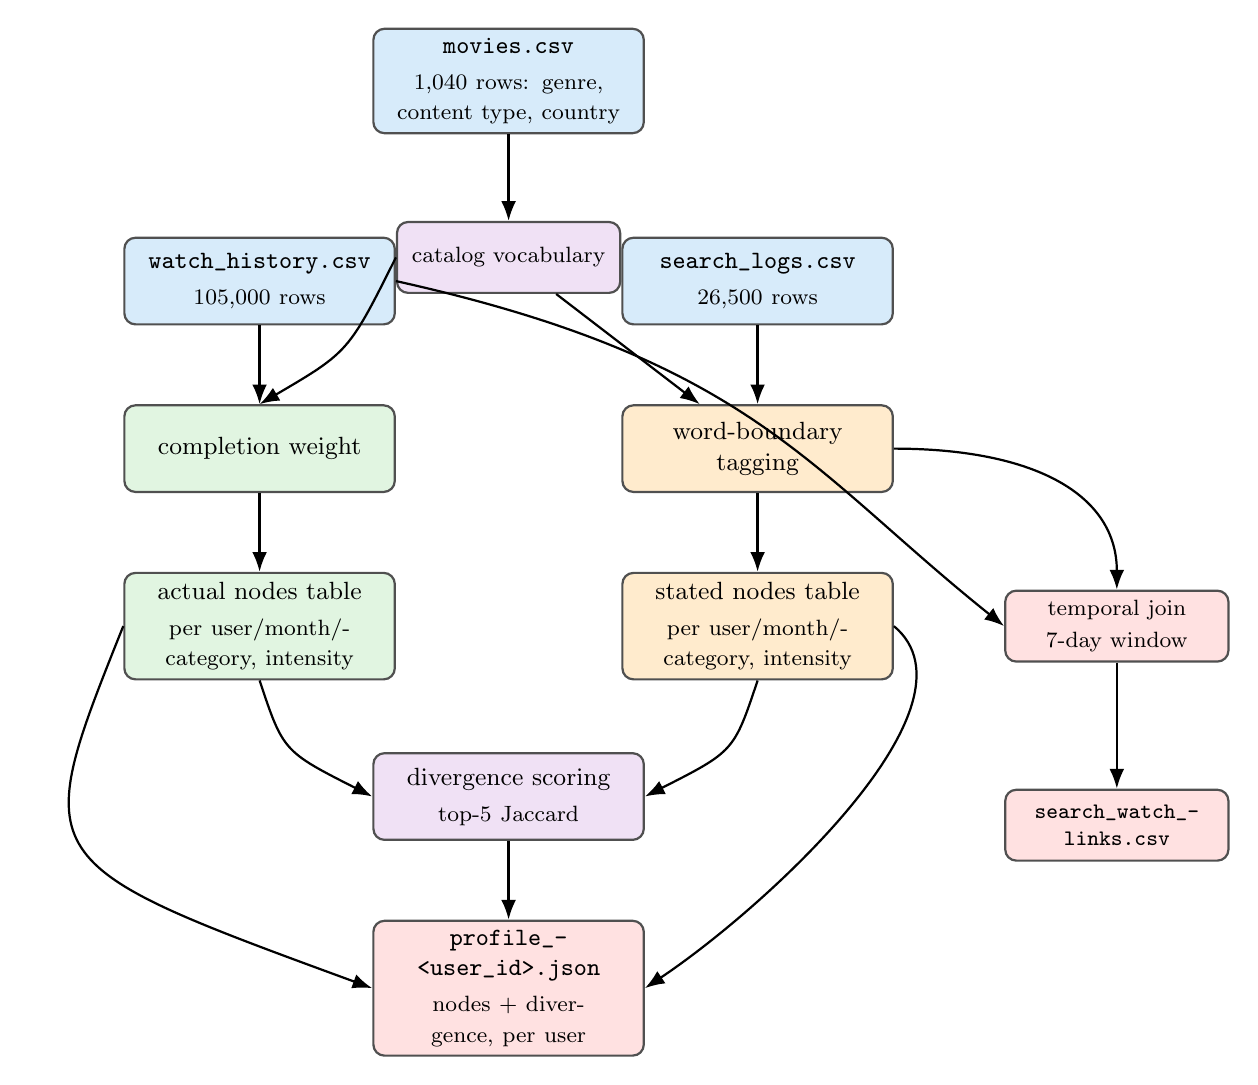
\begin{tikzpicture}[node distance=1.0cm and 1.3cm]

    \node[block, fill=colSource] (movies) {\code{movies.csv}\\[2pt]\footnotesize 1{,}040 rows: genre, content type, country};
    \node[block, fill=colSource, below left=1.3cm and -0.3cm of movies] (watch) {\code{watch\_history.csv}\\[2pt]\footnotesize 105{,}000 rows};
    \node[block, fill=colSource, below right=1.3cm and -0.3cm of movies] (search) {\code{search\_logs.csv}\\[2pt]\footnotesize 26{,}500 rows};

    \node[smallblock, fill=colPurple, below=1.1cm of movies] (vocab) {catalog vocabulary};

    \node[block, fill=colGreen, below=of watch] (weight) {completion weight};
    \node[block, fill=colOrange, below=of search] (tag) {word-boundary tagging};

    \node[block, fill=colGreen, below=of weight] (actualtab) {actual nodes table\\[2pt]\footnotesize per user/month/category, intensity};
    \node[block, fill=colOrange, below=of tag] (statedtab) {stated nodes table\\[2pt]\footnotesize per user/month/category, intensity};

    \node[smallblock, fill=colPink, right=1.4cm of statedtab] (link) {temporal join\\[2pt]\footnotesize 7-day window};

    \coordinate (midAS) at ($(actualtab)!0.5!(statedtab)$);
    \node[block, fill=colPurple, below=1.6cm of midAS] (div) {divergence scoring\\[2pt]\footnotesize top-5 Jaccard};

    \node[block, fill=colPink, below=of div] (out) {\code{profile\_<user\_id>.json}\\[2pt]\footnotesize nodes + divergence, per user};
    \node[smallblock, fill=colPink, below=1.6cm of link] (links) {\code{search\_watch\_links.csv}};

    \draw[arrow] (movies) -- (vocab);
    \draw[arrow] (vocab) -- (tag);
    \draw[arrow] (vocab.west) .. controls +(-0.6,-1.2) .. (weight.north);
    \draw[arrow] (watch) -- (weight);
    \draw[arrow] (search) -- (tag);
    \draw[arrow] (weight) -- (actualtab);
    \draw[arrow] (tag) -- (statedtab);
    \draw[arrow] (tag.east) .. controls +(1.8,0) and +(0,1.2) .. (link.north);
    \draw[arrow] (watch.east) .. controls +(4.5,-1.0) and +(-2.5,2.0) .. (link.west);
    \draw[arrow] (actualtab.south) .. controls +(0.3,-0.9) .. (div.west);
    \draw[arrow] (statedtab.south) .. controls +(-0.3,-0.9) .. (div.east);
    \draw[arrow] (div) -- (out);
    \draw[arrow] (actualtab.west) .. controls +(-1.2,-3.0) .. (out.west);
    \draw[arrow] (statedtab.east) .. controls +(1.2,-1.0) and +(1.5,1.0) .. (out.east);
    \draw[arrow] (link) -- (links);

\end{tikzpicture}
\end{adjustbox}
\caption{The behavioral-profiling pipeline. The catalog vocabulary (top) tags search queries and
implicitly defines the category space watch events are grouped into. The actual (left) and stated
(right) branches each produce a per-user/month/category intensity table, feeding both the per-user
JSON profiles and a divergence score; the temporal join (bottom left) produces a separate,
row-level output.}
\label{fig:behavior-pipeline}
\end{figure}

\section{Results}
\label{sec:behavior-results}

The pipeline was run against the full dataset (Table~\ref{tab:behavior-results}).

\begin{table}[H]
\centering
\begin{tabular}{lr}
\toprule
\textbf{Metric} & \textbf{Value} \\
\midrule
Users with a behavioral profile written & 10{,}000 of 10{,}300 \\
Search$\to$watch links found (7-day window) & 1{,}179 \\
Average stated-vs-actual Jaccard similarity & \textbf{0.01} \\
Users with zero overlap (top-5 stated vs.\ top-5 actual) & \textbf{9{,}399 / 10{,}000} \\
\bottomrule
\end{tabular}
\caption{Behavioral-profiling results on the full dataset. 300 users have no watch history and
therefore receive no profile.}
\label{tab:behavior-results}
\end{table}

As a spot check, one profile was inspected directly: its actual top-5 was \code{["Movie", "USA",
"Canada", "Adventure", "War"]} (a mix of content-type, country, and genre values, since all three
category types share one ranking pool), its stated top-5 was \code{["Action"]} (this user had only
one tagged search in the log), the overlap was empty, and the Jaccard similarity was $0.0$ ---
consistent with the aggregate numbers above. This same user's profile is used again in
Chapter~\ref{ch:recommender} as a worked example of the recommender's behavior in practice.

\section{Interpretation and Limitations}
\label{sec:behavior-limits}

The near-zero average Jaccard similarity ($0.01$) is a striking number, and its \emph{direction} is
consistent with the supervisor's own framing example. It should not, however, be reported as a
validated real-world divergence rate. The underlying dataset is Faker-generated synthetic data with
no true causal link between a search string and a later watch event --- a search and a subsequent
watch being uncorrelated is exactly what random generation would produce, so this number reflects
the heuristic's behavior on synthetic data at least as much as it reflects a real
stated-not-equal-actual phenomenon. This caveat is repeated in Chapter~\ref{ch:eval} because it
directly bounds how strongly that chapter's ablation results can be claimed to generalize.

The 7-day linking window (Section~\ref{sec:behavior-link}) is a heuristic choice, not derived from
the data; a sensitivity check at other window widths was not performed and is noted as future work
(Section~\ref{sec:conclusion-future}). Recency weighting (older watches currently count equally
with recent ones) and review-sentiment as a third signal were also not incorporated, left for a
later iteration if the divergence signal needed refining --- in the event, the signal as built
proved sufficient to produce the clear ablation effect reported in Chapter~\ref{ch:eval}, so this
extension was not pursued.

% =============================================================================
\chapter{The Query Recommender Core}
\label{ch:recommender}
% =============================================================================

This chapter presents the thesis's central design contribution: a four-stage pipeline that turns a
just-answered query, a user's own query history, and their behavioral profile
(Chapter~\ref{ch:behavior}) into three follow-up query suggestions.

\section{Overview}
\label{sec:rec-overview}

The central research question --- can conditioning on real behavior, not just query history,
produce measurably different recommendations --- is operationalized directly in this chapter's
design: the candidate-generation prompt (Section~\ref{sec:rec-generation}) explicitly presents the
LLM with two separate signals, framed as potentially \emph{different} things, not two views of the
same preference; and the ranking stage (Section~\ref{sec:rec-ranking}) makes this signal
load-bearing rather than decorative, rewarding candidates that align with the behavioral profile's
real top categories, not merely with the user's own past phrasing. All four stages are composed
inside the single extension point Section~\ref{sec:arch-api} established,
\code{handle\_recommend()}, requiring no change to the API contract or the development harness.

\begin{figure}[H]
\centering
\begin{adjustbox}{max width=\textwidth, max totalheight=0.88\textheight, center}
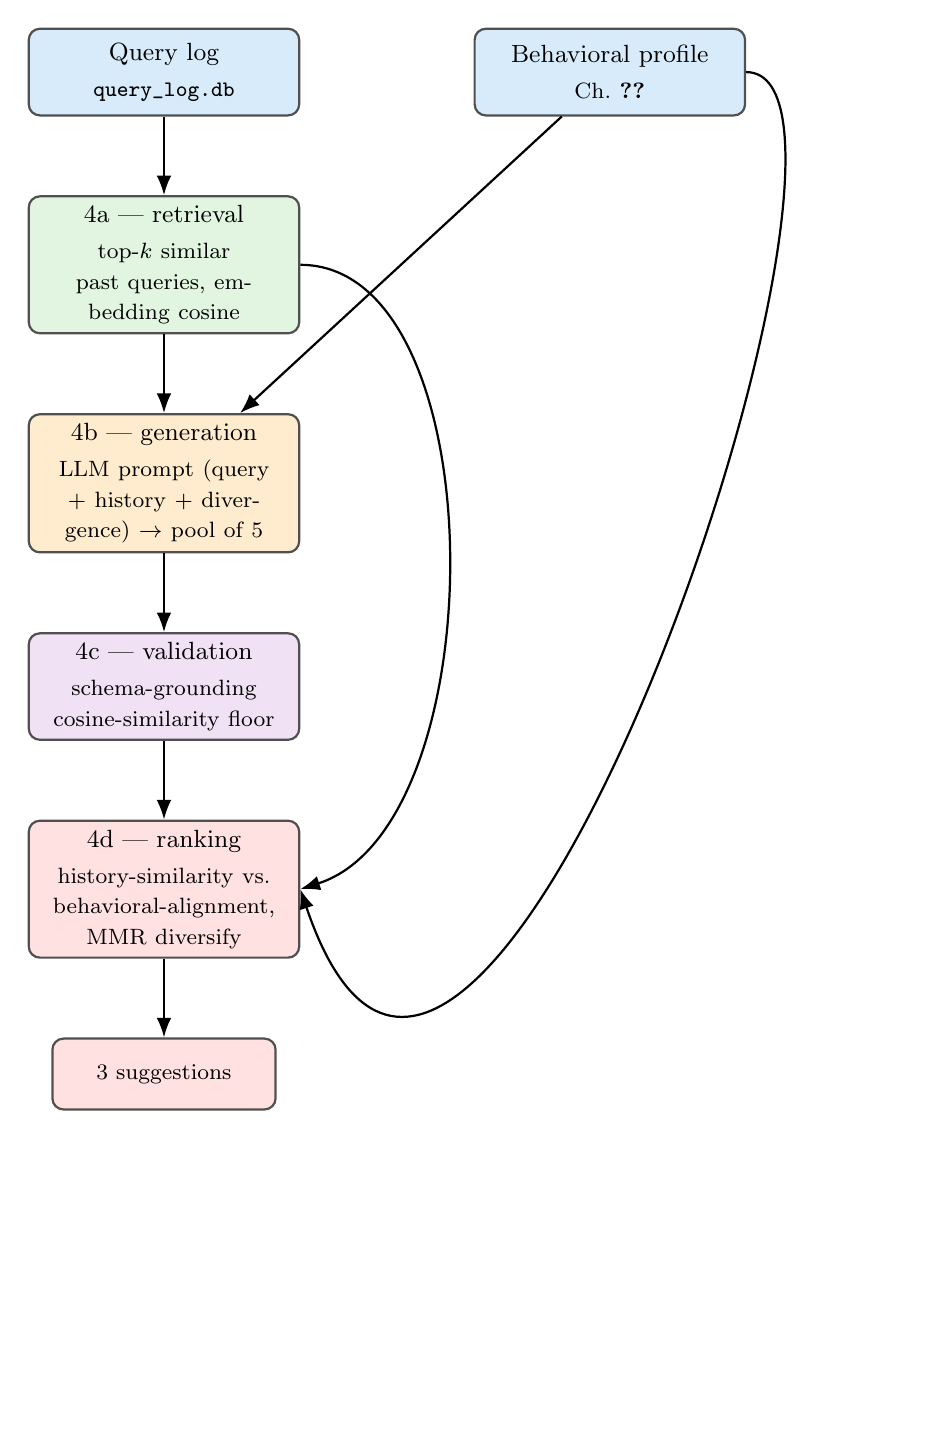
\begin{tikzpicture}[node distance=1.0cm and 2.2cm]

    \node[block, fill=colSource] (qlog) {Query log\\[2pt]\footnotesize \code{query\_log.db}};
    \node[block, fill=colSource, right=of qlog] (bprof) {Behavioral profile\\[2pt]\footnotesize Ch.~\ref{ch:behavior}};

    \node[block, fill=colGreen, below=of qlog] (retrieve) {4a --- retrieval\\[2pt]\footnotesize top-$k$ similar past queries, embedding cosine};

    \node[block, fill=colOrange, below=of retrieve] (generate) {4b --- generation\\[2pt]\footnotesize LLM prompt (query + history + divergence) $\to$ pool of 5};

    \node[block, fill=colPurple, below=of generate] (validate) {4c --- validation\\[2pt]\footnotesize schema-grounding cosine-similarity floor};

    \node[block, fill=colPink, below=of validate] (rank) {4d --- ranking\\[2pt]\footnotesize history-similarity vs.\ behavioral-alignment, MMR diversify};

    \node[smallblock, fill=colPink, below=of rank] (out) {3 suggestions};

    \draw[arrow] (qlog) -- (retrieve);
    \draw[arrow] (retrieve) -- (generate);
    \draw[arrow] (bprof) -- (generate);
    \draw[arrow] (generate) -- (validate);
    \draw[arrow] (validate) -- (rank);
    \draw[arrow] (retrieve.east) .. controls +(2.5,0) and +(2.5,0.8) .. (rank.east);
    \draw[arrow] (bprof.east) .. controls +(2.2,0) and +(2.2,-6.5) .. (rank.east);
    \draw[arrow] (rank) -- (out);

\end{tikzpicture}
\end{adjustbox}
\caption{The four-stage recommender core. The behavioral profile (right) feeds both the generation
prompt and the ranking score directly --- the two concrete points where the thesis's
stated-vs-actual signal shapes the final output, not just the initial candidate pool.}
\label{fig:rec-pipeline}
\end{figure}

\section{Retrieval}
\label{sec:rec-retrieval}

The retrieval stage implements the retrieval half of RA-GQR~\cite{bacciu2024}: a user's query
history is pulled from the query log (Section~\ref{sec:arch-api}), exact duplicates of the current
query are excluded, the current query and every remaining history entry are embedded with the same
sentence-embedding model already used elsewhere in the NL2SPARQL pipeline for class/property
relevance extraction, and candidates are ranked by cosine similarity. The top-$k$ retrieved queries
become the few-shot context for Section~\ref{sec:rec-generation}'s prompt, in place of generically
hand-curated examples. If a user has no other logged queries, the function returns an empty list;
the generation stage still functions correctly, consistent with the original GQR premise that the
technique does not require historical data to work at all.

This stage was verified directly: seeding one user's query log with four varied movie queries, and
querying with \emph{``Show me exciting action films,''} correctly ranked \emph{``Action movies''}
(0.79 cosine) and \emph{``Best action movies with high ratings''} (0.765) above \emph{``Romantic
comedies''} (0.371), excluding unrelated seeded queries entirely.

\section{Candidate Generation}
\label{sec:rec-generation}

A prompt is assembled from three inputs: the current query; the retrieved similar past queries,
rendered as a bulleted list; and a compact rendering of the behavioral divergence
(Section~\ref{sec:behavior-divergence}), explicitly framed as \emph{``what this user says they
want''} versus \emph{``what this user actually engages with, which may DIFFER.''} The LLM is asked
for a pool of \textbf{five} candidates, deliberately more than the three ultimately returned, so
that the validation and ranking stages have real material to filter and diversify from.

Generation reuses the same multi-provider LLM abstraction already used elsewhere in the codebase,
so the recommender can run against any configured provider --- cloud or local --- without code
changes, only an environment variable and that provider's credentials. In practice, both configured
cloud providers (Gemini and OpenAI) turned out to be unusable during this thesis for account and
billing reasons unrelated to the code: one had no billing configured, the other had a zero free-tier
quota on its project. Rather than block on acquiring new credentials, a local, containerized Ollama
model (\code{llama3.1:8b}) was integrated as an additional provider, requiring no API key and no
quota, and was used for all generation reported in this thesis, including the evaluation in
Chapter~\ref{ch:eval}. This is explicitly a validation of the \emph{pipeline}, not of the
\emph{provider} originally envisioned; the abstraction was already provider-agnostic before this
substitution, so a funded cloud key could be swapped in later with no code change. At this
substitution's local, CPU-only configuration, one generation call takes roughly 18--22 seconds ---
acceptable for offline evaluation, but worth flagging as a real deployment-latency concern distinct
from suggestion quality.

\section{Schema-Grounding Validation}
\label{sec:rec-validation}

\subsection{Motivation and original design}

Section~\ref{sec:rel-kgllm} establishes the motivation directly: LLM-generated content referencing
structured knowledge is a documented hallucination risk, and the baseline system's own measured
SPARQL-correctness rate (70\%, Section~\ref{sec:rel-nl2sparql}) is a concrete reminder that this
risk is not merely theoretical in this exact class of system. The original design intent was to run
each candidate query's implied entities and classes through the NL2SPARQL pipeline's own
class-relevance and property-relevance evaluators, confirming a candidate is answerable against the
currently loaded domain schema before it is ever shown to a user.

\subsection{Empirical calibration and a negative result}

Two implementations of this idea were built and empirically rejected before a third, deliberately
weaker version shipped.

The first, reusing the pipeline's own class-relevance evaluator directly, uses relative
thresholding --- keeping every class scoring at or above one standard deviation below the mean
across the schema's own classes. With only 7--11 classes per domain, this reliably selects at least
one class for \emph{any} input, including completely unrelated text: evaluating \emph{``Best pizza
recipe''} against the Tourism schema returned a non-empty class list.

The second computed raw cosine similarity between each candidate and every class's embedded
description, requiring the maximum score across all classes to clear a fixed floor. This was
calibrated against control (clearly off-topic) and probe (genuinely in-domain) phrases
(Table~\ref{tab:rec-calibration}).

\begin{table}[H]
\centering
\begin{tabular}{lclr l}
\toprule
\textbf{Query} & \textbf{Domain} & \textbf{Max cosine sim.} & \textbf{Best-matching class} \\
\midrule
Top rated action movies from the 2010s        & movie    & 0.275 & Movie \\
Movies directed by Christopher Nolan          & movie    & 0.302 & Movie \\
Documentaries produced in Canada              & movie    & 0.288 & Country \\
Best pizza recipe \emph{(control)}            & movie    & 0.175 & SubscriptionPlan \\
How to fix a flat tire \emph{(control)}       & movie    & 0.094 & Country \\
\textbf{Churches in Verona}                   & tourism  & 0.163 & Location \\
\textbf{Roman Churches in Verona}             & tourism  & 0.154 & Location \\
\textbf{Free Churches in Verona}              & tourism  & \textbf{0.092} & Location \\
Events happening this weekend                 & tourism  & 0.401 & Event \\
Art categories available                      & tourism  & 0.601 & ArtCategory \\
Best pizza recipe \emph{(control)}            & tourism  & 0.064 & Tour \\
\textbf{How to fix a flat tire (control)}     & tourism  & \textbf{0.112} & Tour \\
Latest news about the stock market \emph{(control)} & tourism & 0.004 & --- \\
\bottomrule
\end{tabular}
\caption{Absolute cosine-floor calibration data. The Movie domain separates cleanly, but the
Tourism domain does not: the supervisor's own canonical example, \emph{``Free Churches in
Verona,''} scores below an off-topic control phrase.}
\label{tab:rec-calibration}
\end{table}

The Movie domain separates cleanly (in-domain floor $\approx 0.275$, control ceiling $\approx
0.175$). \textbf{The Tourism domain does not}: \emph{``Free Churches in Verona''} --- one of the
supervisor's own three canonical example suggestions, quoted verbatim in the original scoping email
(Section~\ref{sec:intro-motivation}) --- scores $0.092$, below the off-topic control phrase
\emph{``How to fix a flat tire''} at $0.112$. No single threshold can accept the former while
rejecting the latter. A $z$-score variant, relative to each query's own mean and standard deviation
across classes, was also tried and rejected for the same underlying reason: with only 7--11 classes,
the maximum of such a small sample is reliably 1.3--2.3 standard deviations above the mean
regardless of whether the query is on-topic, confirmed empirically --- \emph{``Best pizza recipe''}
against the Movie schema scored a \emph{higher} $z$-score than several genuinely in-domain movie
queries.

The root cause is structural, not a tuning failure: both domains' machine-readable schema class
descriptions are generated purely from SHACL cardinality constraints (e.g.\ \emph{``Art has exactly
1 Art Class ID''}), with no natural-language descriptions and no example instance values in either
source ontology. The Tourism ontology's classes carry essentially no text a general-purpose sentence
embedding could relate to English words like ``church'' --- that correspondence only exists via the
literal Italian category value \emph{``Chiese''} in the live database, which is not present anywhere
in the schema metadata being embedded.

\subsection{What shipped instead}

Given this finding, the shipped validation step uses the absolute-cosine-floor mechanism with a
threshold of $0.05$ --- low enough to reject only genuinely degenerate candidates (near-zero or
negative similarity to every class in the schema, such as \emph{``Latest news about the stock
market''} at $0.004$) while admitting everything else, including borderline-but-valid phrasings like
\emph{``Free Churches in Verona.''} This is explicitly documented as a coarse sanity filter, not the
precision hallucination guard originally intended, and is re-verified against four cases:
\emph{``Free Churches in Verona''} (tourism) and \emph{``Roman Churches in Verona''} (tourism) both
correctly pass; \emph{``Top rated action movies''} (movie) correctly passes; \emph{``Latest news
about the stock market''} (tourism) correctly fails.

This negative result is treated here as a genuine, reportable contribution
(Section~\ref{sec:intro-contrib}) rather than a silently shipped limitation: automatic
schema-grounding of natural-language candidate suggestions, at the class-description level, was not
achievable with acceptable precision given how sparse this project's source ontologies are. A
stronger version would require enriching class descriptions with real catalog/instance values pulled
from the live VKG endpoints --- a concrete, scoped direction for future work
(Section~\ref{sec:conclusion-future}).

\section{Ranking and Diversification}
\label{sec:rec-ranking}

The final stage scores surviving candidates along two axes echoing QRMOCCGA's two-objective framing
(Section~\ref{sec:rel-qrmoccga}), each normalized to $[0,1]$: history-similarity, the maximum
Jaccard word overlap between a candidate and any of the user's retrieved similar past queries; and
behavioral-alignment, the fraction of the behavioral profile's real top interest categories
(Chapter~\ref{ch:behavior}) whose words appear in the candidate text. This second axis is the
concrete place the thesis's central signal enters ranking: a candidate that textually references
what the user \emph{actually watches}, not just what they typed, scores higher here. A weighted sum
of the two axes ranks the candidate pool; a greedy, Maximal-Marginal-Relevance-style loop then
repeatedly selects the highest-scoring remaining candidate, penalized by its word overlap with
candidates already selected, so the final three suggestions are not near-duplicates of one another.

This stage was verified with a hand-built pool of five candidates (one near-duplicate of query
history, two behaviorally-aligned, one off-axis, one more history-similar): it correctly picked the
history-similar candidate first, then diversified into the two behaviorally-aligned candidates
rather than a near-duplicate of the first pick. Reimplementing QRMOCCGA's cooperative
co-evolutionary genetic algorithm itself was explicitly out of scope --- only its feature ideas were
borrowed, as planned in Section~\ref{sec:rel-qrmoccga}.

\section{End-to-End Verification}
\label{sec:rec-verification}

The full chain was verified at three levels of fidelity. First, with a mocked LLM returning fixed
candidates, the real production entry point --- not a reimplementation --- was called for the
user profiled in Section~\ref{sec:behavior-results} with the query \emph{``Show me exciting action
films.''} The result:

\begin{lstlisting}[language=, caption={Mocked-LLM end-to-end output, ranked top to bottom.}]
War documentaries produced in the USA
Crime thrillers with high ratings
Adventure movies set during wartime
\end{lstlisting}

The top-ranked suggestion is the one most strongly aligned with this user's \emph{actual} top
interest categories (\code{Movie, USA, Canada, Adventure, War}) rather than a plain paraphrase of
the stated query about ``action films.''

Second, over real HTTP with a placeholder API key, the server log confirmed the full path executed
--- log, retrieval, a generation attempt that failed cleanly on the invalid key, caught and logged
as a warning rather than a crash --- and the response was \code{200 OK} with an empty suggestion
list, confirming the pipeline degrades gracefully rather than failing the request when generation is
unavailable.

Third, and most significantly, against genuine Ollama-backed model output (Section~\ref{sec:rec-generation}),
the same request produced:

\begin{lstlisting}[language=, caption={End-to-end suggestions from genuine \code{llama3.1:8b}
output, via the real production code path.}]
{
  "suggestions": [
    "War movies with high ratings on IMDB",
    "Movies that combine action and adventure genres",
    "Films starring actors from Canada or USA"
  ]
}
\end{lstlisting}

All three suggestions reference this user's real \code{actual\_top} categories, not a paraphrase of
the stated query --- reproducing, with genuine model output, the same qualitative pattern already
observed with the mocked-LLM run.

\section{Interpretation and Limitations}
\label{sec:rec-limits}

The schema-grounding check (Section~\ref{sec:rec-validation}) is intentionally weak, and is reported
as such rather than presented as the precision filter originally planned. The candidate pool size
(five) is an arbitrary choice, not derived from data; a sensitivity check across pool sizes was not
performed. The behavioral-alignment ranking axis only functions for the Movie domain today, since
behavioral profiles only exist there (Section~\ref{sec:arch-vkgs}); it correctly returns $0.0$ when
no profile exists, so Tourism recommendations degrade to history-similarity-only ranking rather than
erroring, but this means the thesis's core stated-vs-actual contribution is only demonstrable
end-to-end on the Movie domain --- consistent with every earlier chapter's own scoping note. A
systematic, quantitative check of suggestion quality across many users and queries, rather than the
worked examples in Section~\ref{sec:rec-verification}, is the subject of Chapter~\ref{ch:eval}.

% =============================================================================
\chapter{Evaluation}
\label{ch:eval}
% =============================================================================

\section{Methodology}
\label{sec:eval-method}

Chapter~\ref{ch:recommender} verified the recommender \emph{qualitatively}, on worked examples. This
chapter turns that into a controlled, quantitative comparison, answering four questions: does the
schema-grounding step let anything sensible through at all; does adding the behavioral signal shift
suggestions in the intended direction; would the resulting suggestions have actually surfaced
content the user went on to watch; and how does a trivial, non-LLM baseline compare on the same
metrics. All four are answered by running the real, unmodified recommender core from
Chapter~\ref{ch:recommender} --- no reimplementation, no mocking --- with an evaluation harness
layered additively on top of it. The evaluation scope was deliberately kept small: 3 Movie users
$\times$ 4 test questions $\times$ 2 ablation conditions (24 LLM calls), plus 4 Tourism test
questions (4 calls).

An honest ablation requires that the two compared conditions differ \emph{only} in the variable
under test, and that both are graded against the same, uncontaminated ground truth. This is
achieved with three mechanisms. First, evaluation users are selected among those with a behavioral
profile, at least five search-log rows, and \emph{maximal} stated-vs-actual divergence (zero
Jaccard similarity), for the sharpest possible contrast; the first three by user id are used for
reproducibility. Second, each selected user's behavioral profile is rebuilt \emph{held out}: watch
history is split at that user's own 80th-percentile watch date, everything at or before the cutoff
building a held-out profile the recommender is allowed to see, everything after kept aside as proxy
ground truth --- and the same cutoff bounds which search-log rows seed retrieval, so no future
information leaks into either signal. Third, query-history retrieval is seeded from this held-out
data via a new optional parameter on the retrieval function, entirely bypassing the shared
production query log, so the live system used by real callers is untouched by the evaluation run.

\begin{figure}[H]
\centering
\begin{adjustbox}{max width=\textwidth, max totalheight=0.88\textheight, center}
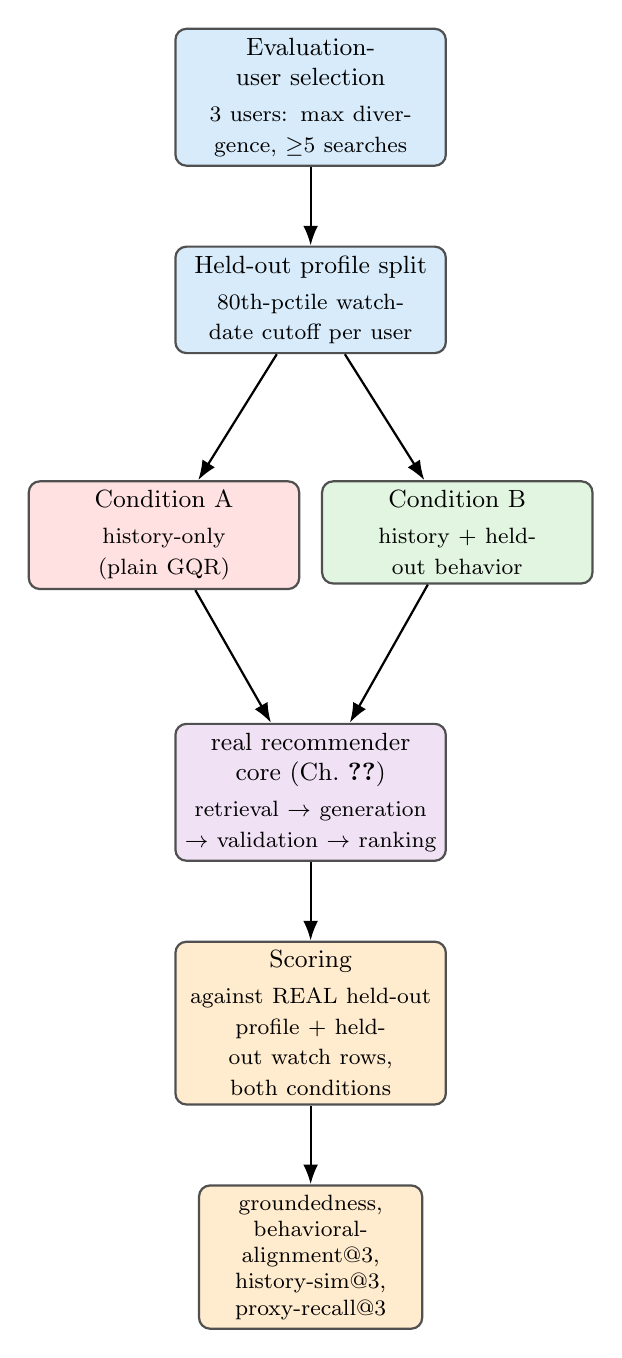
\begin{tikzpicture}[node distance=1.0cm and 1.5cm]

    \node[block, fill=colSource] (users) {Evaluation-user selection\\[2pt]\footnotesize 3 users: max divergence, $\geq$5 searches};

    \node[block, fill=colSource, below=of users] (split) {Held-out profile split\\[2pt]\footnotesize 80th-pctile watch-date cutoff per user};

    \node[block, fill=colPink, below left=1.6cm and -1.6cm of split] (condA) {Condition A\\[2pt]\footnotesize history-only (plain GQR)};
    \node[block, fill=colGreen, below right=1.6cm and -1.6cm of split] (condB) {Condition B\\[2pt]\footnotesize history + held-out behavior};

    \coordinate (midCond) at ($(condA)!0.5!(condB)$);
    \node[block, fill=colPurple, below=2.4cm of midCond] (chain) {real recommender core (Ch.~\ref{ch:recommender})\\[2pt]\footnotesize retrieval $\to$ generation $\to$ validation $\to$ ranking};

    \node[block, fill=colOrange, below=of chain] (score) {Scoring\\[2pt]\footnotesize against REAL held-out profile + held-out watch rows, both conditions};

    \node[smallblock, fill=colOrange, below=of score] (out) {groundedness, behavioral-alignment@3,\\ history-sim@3, proxy-recall@3};

    \draw[arrow] (users) -- (split);
    \draw[arrow] (split) -- (condA);
    \draw[arrow] (split) -- (condB);
    \draw[arrow] (condA) -- (chain);
    \draw[arrow] (condB) -- (chain);
    \draw[arrow] (chain) -- (score);
    \draw[arrow] (score) -- (out);

\end{tikzpicture}
\end{adjustbox}
\caption{The evaluation's ablation flow. Both conditions run the identical, real recommender-core
functions; the only difference is whether the behavioral profile is passed. Scoring is decoupled
from what each condition was allowed to see --- both are graded against the same real held-out
ground truth.}
\label{fig:eval-pipeline}
\end{figure}

For every (user, question) pair, the real pipeline is run twice: \textbf{Condition A}
(history-only, plain GQR) with no behavioral profile passed to generation or ranking; and
\textbf{Condition B} (history + behavior) with the held-out profile passed through. Every resulting
suggestion set from both conditions is scored against the same real held-out profile and held-out
watch rows, using the same behavioral-alignment and history-similarity functions
Section~\ref{sec:rec-ranking} already uses for ranking, plus a new proxy-recall check (token overlap
between a suggestion and the held-out rows' genre/country/content-type values). A trivial, non-LLM
classical baseline, mirroring both the frequency-based fallback in the baseline system and
QRMOCCGA's non-LLM framing without reimplementing either paper's actual method, returns up to three
suggestions of the form ``\{category\} movies,'' one per profile's top category.

\section{Results}
\label{sec:eval-results}

\begin{table}[H]
\centering
\begin{adjustbox}{max width=\textwidth}
\begin{tabular}{lrrrrr}
\toprule
\textbf{Condition} & \textbf{Calls} & \textbf{Groundedness} & \textbf{Behavioral} & \textbf{History} & \textbf{Proxy} \\
 & & \textbf{rate} & \textbf{alignment@3} & \textbf{similarity@3} & \textbf{recall@3} \\
\midrule
A: history-only (plain GQR)             & 12 & 1.00 & \textbf{0.022} & 0.121 & \textbf{0.25} \\
B: history + behavior (this thesis)     & 12 & 1.00 & \textbf{0.144} & 0.057 & \textbf{0.583} \\
Classical baseline (non-LLM template)   & 3  & 1.00 & 0.222          & ---    & 1.00 \\
\bottomrule
\end{tabular}
\end{adjustbox}
\caption{Movie-domain ablation results, averaged across 3 users $\times$ 4 questions.}
\label{tab:eval-ablation}
\end{table}

\textbf{The headline result}: Condition B's behavioral-alignment@3 is approximately $6.5\times$
Condition A's ($0.144$ vs.\ $0.022$), and its proxy-recall@3 is more than double ($0.583$ vs.\
$0.25$) --- the direct, quantitative confirmation of this thesis's central claim, consistent across
every one of the three evaluated users and all four test questions, not a cherry-picked case.

An unexpected, worth-reporting side effect: history-similarity@3 is \emph{lower} in Condition B
($0.057$) than Condition A ($0.121$). Adding the behavioral signal does not simply layer new
information on top of the history-only suggestions --- it visibly \emph{displaces} some of the
lexical closeness to the user's own past queries in favor of behaviorally novel suggestions, a
genuine trade-off rather than a free lunch (Section~\ref{sec:eval-qual}).

The classical baseline's very high behavioral-alignment@3 ($0.222$) and perfect proxy-recall@3
($1.00$) are close to definitional, not a fair ``it beats the LLM'' result: its suggestions are
literally the profile's own top category names, so scoring them against that same profile's
categories is close to tautological. It is included as a required sanity ceiling and a legitimate
non-LLM comparison point, not as evidence the LLM-based approach underperforms --- Condition B,
notably, still generates novel, well-formed natural-language queries rather than a category name
mechanically appended with ``movies.''

No behavioral profile exists for Tourism, by the design decision recorded in
Section~\ref{sec:arch-vkgs}, so the ablation and proxy-recall metrics do not apply there. A
groundedness-only check on four Tourism test questions (20 raw candidates across all four) passed
$0.95$ of candidates through the schema-grounding filter --- consistent with that filter's
documented design as a weak sanity check (Section~\ref{sec:rec-validation}) rather than a precision
guard: a near-100\% pass rate confirms the filter is not degenerate, but says nothing further about
precision.

\section{Qualitative Examples}
\label{sec:eval-qual}

Two representative rows illustrate the mechanism behind Table~\ref{tab:eval-ablation}'s numbers.

\paragraph{One user, query ``Show me exciting action films''} (actual-top categories: Horror, USA,
TV Series, Canada --- not Action, despite the stated query).
\begin{itemize}
    \item \textbf{A}: \emph{``What are the most popular action movies on Netflix,'' ``Can you
        recommend some intense martial arts films,'' ``Show me action films starring Dwayne
        Johnson''} --- straightforward elaborations of ``action,'' ignoring behavior entirely.
    \item \textbf{B}: \emph{``Horror movies on Netflix,'' ``USA action films of the 80s,''
        ``Canadian TV series based on true stories''} --- visibly pivots toward Horror/USA/Canada,
        the user's real top-watched categories, while still keeping one action-adjacent suggestion.
\end{itemize}

\paragraph{Another user, query ``What movies have the genre Action?''} (actual-top: USA, Stand-up
Comedy, Documentary, Comedy --- again, not Action).
\begin{itemize}
    \item \textbf{A}: \emph{``...family-friendly action movies?,'' ``Movies similar to Die
        Hard...,'' ``...action movies with a strong female lead?''} --- all still literally about
        action movies.
    \item \textbf{B}: \emph{``Stand-up comedians who have acted in movies,'' ``Movies similar to
        Die Hard,'' ``Action movies set in New York City''} --- one suggestion pivots fully to
        stand-up comedy, this user's actual top category; a second stays closer to the stated query.
\end{itemize}

\section{Threats to Validity and Limitations}
\label{sec:eval-limits}

Sample size is small, by explicit choice (3 users, 4 questions, 12 scored suggestion sets per
condition). The direction and magnitude of the ablation effect ($6.5\times$ alignment, $2.3\times$
proxy recall) are large enough to be a credible signal at this size, but a larger run --- more
users, more questions, supported by the harness with no code changes --- would strengthen these
claims statistically, and is the most direct piece of future work
(Section~\ref{sec:conclusion-future}). Held-out watch rows are very few per user (1--3 rows), an
artifact of the per-user percentile cutoff applied to a modest amount of synthetic watch history;
proxy-recall numbers should be read as directionally informative, not statistically tight.

The synthetic-data caveat from Chapter~\ref{ch:behavior} carries over directly: the underlying
dataset has no real causal link between a stated search and a later watch, so the specific
\emph{magnitude} of the divergence effect is a property of this dataset's generation process as
much as of real user behavior. This directly bounds how strongly these results can be claimed to
generalize to real users; re-running this exact harness against real interaction data, if it ever
becomes available, is a direct, no-code-change validation step.

This evaluation used a local Ollama model rather than the originally-planned cloud provider
(Section~\ref{sec:rec-generation}); re-running after flipping the provider is a direct,
no-code-change comparison worth pursuing if a funded key becomes available, to check whether
suggestion quality or alignment changes with a stronger model.

% =============================================================================
\chapter{Conclusion and Future Work}
\label{ch:conclusion}
% =============================================================================

\section{Summary of Contributions}
\label{sec:conclusion-summary}

This thesis set out to answer a specific research question, posed directly by the supervisor: can a
query recommender that conditions on both a user's stated queries and their real interaction
behavior produce measurably better follow-up suggestions than one conditioning on query history
alone? The answer, established in Chapter~\ref{ch:eval}, is yes: a controlled ablation, run on the
real production recommender and scored against real held-out ground truth, shows a $6.5\times$
increase in behavioral-alignment@3 and a more than $2\times$ increase in proxy-recall@3 when the
behavioral signal is included, consistently across every evaluated user and question.

Reaching that result required, in order: a per-user behavioral divergence signal engineered from two
data sources that share no natural key (Chapter~\ref{ch:behavior}); a retrieval-augmented,
LLM-based candidate-generation step conditioned on that signal (Section~\ref{sec:rec-generation});
and a ranking stage that makes the signal load-bearing in the final output
(Section~\ref{sec:rec-ranking}). One design goal, however, was pursued and found not to be
achievable within this thesis's scope: a precision schema-grounding filter, motivated by a
well-documented hallucination risk in the LLM+KG literature, was calibrated against this project's
actual ontologies and found unable to separate the supervisor's own canonical example query from an
off-topic control phrase, because the underlying schema metadata is too sparse for embedding
similarity to carry the necessary signal. This is reported as a concrete, empirically-grounded
negative result (Section~\ref{sec:rec-validation}) rather than an over-claimed feature.

\section{Limitations}
\label{sec:conclusion-limits}

Three limitations bound how far this thesis's results can be claimed to generalize, beyond those
already discussed in each chapter. First, all quantitative results are obtained on a single,
synthetic, Faker-generated dataset with no true causal link between stated search intent and later
watch behavior; the \emph{direction} of the observed divergence and ablation effects is consistent
with the supervisor's own real-world framing, but their \emph{magnitude} is, in part, a property of
this dataset's generation process. Second, per the scope decision in
Section~\ref{sec:arch-vkgs}, the entire behavioral, stated-vs-actual contribution is demonstrable
only on the Movie domain; the Tourism domain's only large behavioral signal is anonymous and was
deliberately excluded. Third, the recommender's input-contract dependency on an external
application --- what real interaction data a caller actually logs per user --- was never resolved
during this thesis; the \code{interaction\_data} field in the API contract
(Section~\ref{sec:arch-api}) remains an untyped placeholder, and all behavioral conditioning in this
work instead uses the offline, precomputed profile described in Chapter~\ref{ch:behavior}.

\section{Future Work}
\label{sec:conclusion-future}

Several concrete extensions follow directly from limitations identified in this thesis, rather than
being open-ended:

\begin{itemize}
    \item \textbf{A larger evaluation run.} Chapter~\ref{ch:eval}'s ablation used 3 users and 4
        questions by explicit scope choice; the evaluation harness already supports a larger run via
        configuration constants alone, with no design or code changes required.
    \item \textbf{Validation against real interaction data.} If the external application's logging
        contract is ever confirmed (Section~\ref{sec:conclusion-limits}), or if any other source of
        real user interaction data becomes available, both the behavioral-profiling pipeline
        (Chapter~\ref{ch:behavior}) and the evaluation harness (Chapter~\ref{ch:eval}) can be
        re-run against it directly, since both already consume this exact CSV schema; this would
        directly test whether the divergence effect's magnitude, not just its direction, holds
        outside synthetic data.
    \item \textbf{Enriching schema metadata for a real precision grounding filter.} The negative
        result in Section~\ref{sec:rec-validation} traces to sparse class descriptions in the source
        ontologies; enriching them with real catalog/instance values pulled from the live VKG
        endpoints is a concrete, scoped path toward the precision hallucination filter originally
        intended.
    \item \textbf{A sensitivity analysis on heuristic parameters.} The temporal-join window
        (Section~\ref{sec:behavior-link}) and the candidate-pool size
        (Section~\ref{sec:rec-generation}) are both fixed, undertuned choices; a systematic sweep
        over both was left for future work once real interaction data makes such tuning meaningful.
    \item \textbf{Re-evaluating against a funded cloud LLM.} All generation and evaluation in this
        thesis used a local Ollama model after both configured cloud providers were blocked by
        account issues unrelated to the code; re-running with a stronger, funded model is a direct,
        no-code-change comparison worth pursuing.
\end{itemize}

% =============================================================================
\backmatter

\begin{thebibliography}{9}

\bibitem{balasooriya2026}
I.~Balasooriya, A.~Dalla Vecchia, and E.~Quintarelli.
\textit{Towards Natural Language Reasoning and Hybrid Querying over Virtual Knowledge Graphs.}
ADBIS 2026.

\bibitem{bacciu2024}
A.~Bacciu, E.~Palumbo, A.~Damianou, N.~Tonellotto, and F.~Silvestri.
\textit{Generating Query Recommendations via LLMs.}
IR-RAG @ SIGIR 2024.

\bibitem{pan2024}
S.~Pan, L.~Luo, Y.~Wang, C.~Chen, J.~Wang, and X.~Wu.
\textit{Unifying Large Language Models and Knowledge Graphs: A Roadmap.}

\bibitem{barman2024}
D.~Barman, R.~Sarkar, and N.~Chowdhury.
\textit{A Cooperative Co-evolutionary Genetic Algorithm for Query Recommendation.}
Multimedia Tools and Applications, 2024.

\bibitem{ontop}
Ontop --- Virtual Knowledge Graph system. \url{https://ontop-vkg.org}

\end{thebibliography}

\end{document}
